\documentclass[a4j, titlepage]{jarticle}

%% プリアンブル部 %%
\usepackage[table]{xcolor}
\usepackage{xurl}
\usepackage{ascmac}
\usepackage[dvipdfmx]{graphicx}
\usepackage{listings}
\usepackage{comment}
\usepackage{fancybox,ascmac}
\usepackage[most]{tcolorbox}
\usepackage{xcolor}

\definecolor{mGreen}{rgb}{0,0.6,0}
\definecolor{mGray}{rgb}{0.5,0.5,0.5}
\definecolor{mPurple}{rgb}{0.58,0,0.82}
\definecolor{backgroundColour}{rgb}{0.95,0.95,0.92}

\lstdefinestyle{CStyle}{
    backgroundcolor=\color{backgroundColour},   
    commentstyle=\color{mGreen},
    keywordstyle=\color{magenta},
    numberstyle=\tiny\color{mGray},
    stringstyle=\color{mPurple},
    basicstyle=\footnotesize,
    frame=TB,
    xleftmargin=\parindent,
    breakatwhitespace=false,        
    breaklines=true,                 
    captionpos=b,                    
    keepspaces=true,                 
    numbers=left,                    
    numbersep=5pt,                  
    showspaces=false,                
    showstringspaces=false,
    showtabs=false,                  
    tabsize=2,
    language=C
}

\title{情報工学実験II\\シムレーションプログラム}
\author{ライモン ウィジャヤ}
\date{2021-06-30}
\begin{document}
\maketitle
\tableofcontents
\clearpage


\section{概要}
乱数とはある範囲の数値から任意に取り出した数値. 
プログラミング言語では, 種(seed)と呼ばれる値を基にして乱数を取り出す関数が用意されている. 
しかし種を定数にしてしまうと, 関数を呼び出すごとに同じ値を乱数としてしまうため, 常に変化する時刻(秒)などを種として利用する. 
それで, Listing\ref{srand}に示した通り, Cプログラムには大事である. そのコードはメイン関数に置く. 
\vspace{20pt}
\begin{lstlisting}[
    style=CStyle,
    caption=CにSeedの値を与える関数,
    captionpos=t,
    label=srand]
int main(void){ 
...
srand((unsigned int)time(NULL));
...
return 0;
}
\end{lstlisting}

\section{サイコロのシムレーション}
今回のシムレイションは6個のサイコロを同時に振とき,全部が同じ出目になる確率を求める. 
実行回数を調整し, 論理値の確率と関係を調べる.
実行回数は$10000, 20000, 40000, \cdots , 81920000$まで行った.

\subsection{コードリスト}
Listing \ref{dice}はdice.cのコードリストである. 実行するとき一つパラメータが必要. そのパラメータは回数の値である. \vspace{10pt}
\begin{lstlisting}[
    style=CStyle, 
    caption=dice.cコードリスト,
    captionpos=t,
    label=dice]
#include <stdio.h>
#include <stdlib.h>
#include <time.h>
#include <unistd.h>
#include <math.h>

#define diceEye 6
#define totaldice 6
#define DEBUG 0

int roll(int a[], int* b);
int randnum();

int main(int argc, char *argv[]){

    if(argc != 2){              
        puts("Parameter Error");
        return 0;
    }

    int N = atoi(argv[1]);
    
    int i;
    int dice[6];
    int TotalSame = 0;
    int success;
    srand((unsigned int)time(NULL));

    for(i = 0; i < N; i++){
        success = roll(dice, &TotalSame);  

        if (success == 1){
#if DEBUG == 1
            printf("%d %d %d %d %d %d \n", dice[0], dice[1], dice[2], dice[3], dice[4], dice[5]);
            //sleep(2);
#endif
        }

    }
    printf("%d %d %lf %e\n", TotalSame, N, (double)TotalSame/(double)N, fabs(((double)1/(double)7666) - (double)TotalSame/(double)N));
    return 1;
}


int roll(int dice[], int* TotalSame)
{
    int i;
    int isSame = 1;

    dice[0] = rand()%6 + 1;

    for(i = 1; i <= totaldice - 1; i++){
        dice[i] = randnum();
        if(dice[0] == dice[i]) isSame++;
    }

    if (isSame == totaldice){
        *TotalSame += 1;
        return 1;
    }
    return 0;
}

int randnum(){
    return rand()%diceEye + 1;
}
\end{lstlisting}
\pagebreak
\subsection{6サイコロが同じ値確率}
実験結果は図\ref{graph:random1}に掲載された. グラフを見ると, 回数を増加させると, 精度が上がっていくということがわかる. つまり理論値に近づいていくということである. また,図\ref{graph:random-gosa}を見ると, 実験値と理論値の誤差がゼロに近づいていくというのは, 理論値に近づくということである.

\begin{figure}[tbh]
    \centering \includegraphics[height=5.4cm, keepaspectratio]{random1.png}
    \caption{回数-実験結果グラフ}
    \label{graph:random1}
\end{figure}

\begin{figure}[tbh]
    \centering \includegraphics[height=5.4cm, keepaspectratio]{random2.png}
    \caption{誤差グラフ}
    \label{graph:random-gosa}
\end{figure}


\section{円率によるシムレーション}
このシムレイションはランダム関数を用い, 半径7の円の面積を求めるというシムレイションである. 理論値は$49\pi$である.
ランダムの点で面積を決める方法は
\[49 : \frac{49\pi}{4} = (in + out) : in \] 
\[49\pi = \frac{196 \times in}{in + out}\]    
である. Listing \ref{code-area}はシムレイションのコードリストである.
\subsection{コードリスト}
\begin{lstlisting}[
    style=CStyle, 
    caption=area.cコードリスト,
    captionpos=t,
    label=code-area]
#include<stdio.h>
#include<stdlib.h>
#include<unistd.h>
#include<math.h>
#include<time.h>
#define RADIUS 7
#define DEBUG 0

int main(int argc, char *argv[]){

    if(argc != 2){              
        puts("Parameter Error");
        return 0;
    }

    int N = atoi(argv[1]);    
    double x, y;
    int in, out;
    int i;
    long double resofArea, resofRealArea, gosa;
    
    in  = 0;
    out = 0;
    srand((unsigned int)time(NULL));

    for(i = 0; i < N; i++){
        x = ((float)rand()/(float)(RAND_MAX)) * RADIUS;
        y = ((float)rand()/(float)(RAND_MAX)) * RADIUS;

        if(x * x + y * y <= RADIUS*RADIUS) {
            in+=1;
        } else {
            out+=1;
        }
    }

    resofArea = (long double)(196*in) / (long double)(in+out);
    resofRealArea = 49.0 * M_PI;
    gosa = fabs(resofArea - resofRealArea);
    printf("%d %Lf %Lf\n", N, resofArea, gosa);
    return 0;
}
\end{lstlisting}
\subsection{実験結果の比較}
実験では1000回数から$1.0 x 10^7$回数までで, 毎回数は10回を行い, 平均を取る. 結果はグラフ\ref{graph:area}に記載されている.
\begin{figure}[tbh]
    \centering 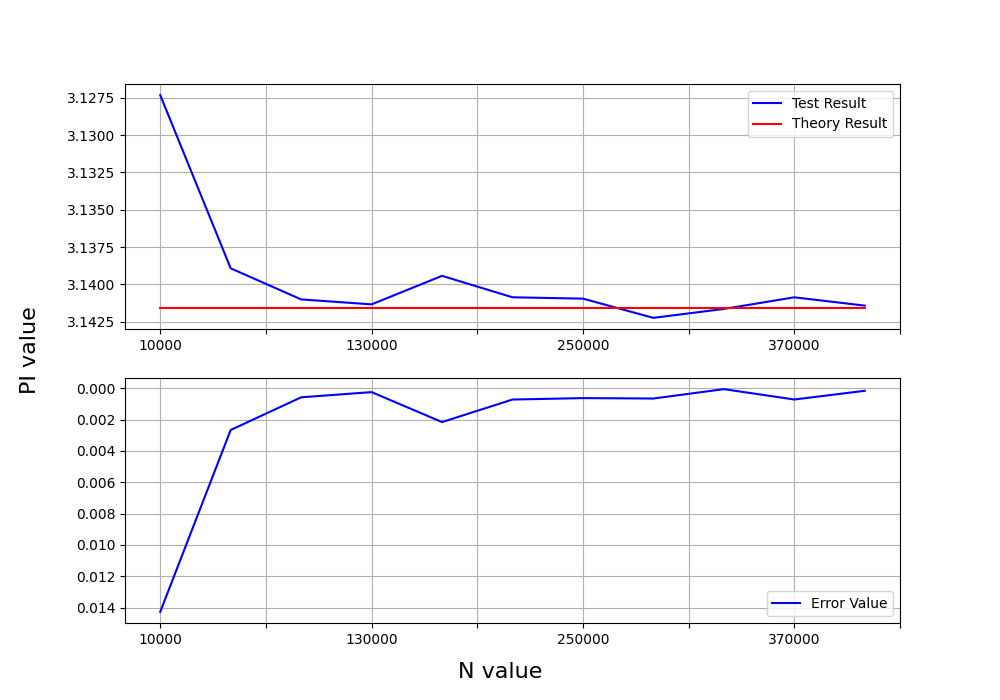
\includegraphics[height=5.4cm, keepaspectratio]{area1.png}
    \caption{回数-実験結果グラフ}
    \label{graph:area}
\end{figure}
誤差値から見ると, グラフ\ref{graph:area2}に記載されている.
\begin{figure}[tbh]
    \centering 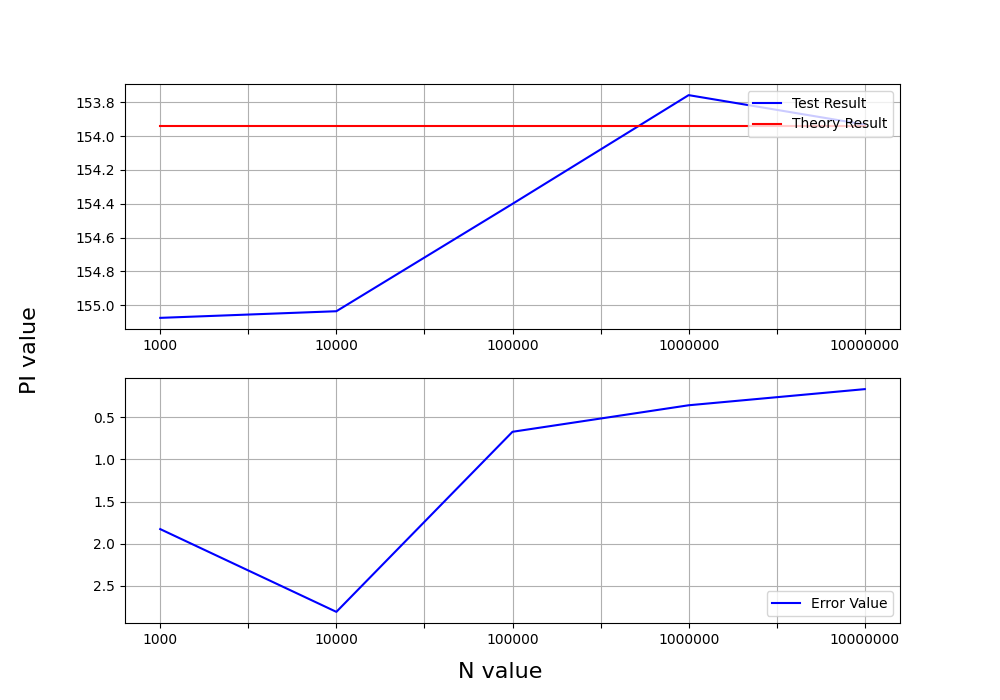
\includegraphics[height=5.4cm, keepaspectratio]{area2.png}
    \caption{回数-誤差グラフ}
    \label{graph:area2}
\end{figure}
グラフ\ref{graph:area}から見ると,実験値は理論値に近づくということが言える. 誤差の値は回数を増加するともに減少するということがわかる. つまり回数がもっと増加されると理論値にもっと近づけるということがわかる. 
\pagebreak
\section{ルーレットシムレーション}
このシムレイションは900ドールを持つとし, 1ドールずつ賭け, 1000ドールに達成する確率を求めるというシムレイションである. ルーレットで赤か黒に入る確率はそれぞれ9/19とする. 今回の実験ではずっと同じ色で賭け, シムレイションする.

\subsection{コードリスト}
Listing \ref{roul}はroulette.cのコードリストである. 実行するとき一つパラメータが必要. そのパラメータは回数の値である. 

\begin{lstlisting}[
    style=CStyle, 
    caption=roullete.cコードリスト,
    captionpos=t,
    label=roul]
#include<stdio.h>
#include<stdlib.h>
#include<unistd.h>
#include<math.h>
#include<time.h>
#define TARGET 1000
#define PROB 9.0/19.0


int main(int argc, char *argv[]) 
{
    if(argc != 2){              
        puts("Parameter Error");
        return 0;
    }

    int N = atoi(argv[1]);
    FILE* fp1;
    int money;
    int win, lose;
    int i, iter;
    double hantei;

    fp1 = fopen("kekka/roul.csv","a+");
    win = lose = 0;
    srand((unsigned int)time(NULL));
        iter = 0;

    for(i = 0; i < N; i++){
        money = 900;
        while(money < TARGET && money > 0){
            hantei = (double)rand() / RAND_MAX;
            if(hantei < PROB) money++;
            else money--;    
        }
        if(money>=TARGET)win++;
        else lose++;
        iter++;
        if(iter % 10000 == 0){
            printf("N[%d]\tkaisuu[%d]\titer[%d]\n", N, i, iter);
            iter = 0;
        }
    }
    
    fprintf(fp1, "%d %d %d \n", N, win, lose);
    fclose(fp1);

}
\end{lstlisting}

\subsection{1000ドールに達成確率}
プログラムを毎回数を10回を行い, 達成した結果の平均を取り, 結果は表\ref{table:roul}に掲載されている.
結果を見ると, 回数を2倍にし, 達成結果は安定に2倍になるということがわかる. この結果を用い, 「64000ゲームの中で最低1か2か1000ドールに達成することができる」という要約である.

\begin{table}[bth]
    \label{table:roul}
    \caption{実験結果}
    \begin{center}
    \begin{tabular}{|l|c||l|c|}
    \hline
    回数 & 達成 & 回数 & 達成 \\ \hline
     64000 &  1.6 & 1024000 &  26.7 \\ \hline
    128000 &  3.3 & 2048000 &  56.4 \\ \hline
    256000 &  6.2 & 4096000 & 107.2 \\ \hline
    512000 & 13.4 & 8192000 & 220.0 \\ \hline
\end{tabular}
\end{center}
\end{table}
\section{並びシムレーション}
このシムレイションは5人男子と5人女子を横に1列に並べるとき, 各女子の左に自身より背の高い男子が1人でもいる並びになると確率を求めるというシムレイションである. 背は \textit{M1} > \textit{W1} > \textit{M2} > \textit{W2} > \textit{M3} > \textit{W3} > \textit{M4} > \textit{W4} > \textit{M5} > \textit{W5} とし,条件より二つ判定が加えることができる.
\begin{enumerate}
    \item 一番左に男子(M1)が来たら,確実に正しい.
    \item 一番左に女子(\textit{W5}, \textit{W4}, \textit{W3}, \textit{W2},\textit{W1})が来たら, 確実に違う.
\end{enumerate}

\subsection{プログラム}
Listing \ref{height}はheight.cのコードリストである. 実行するとき一つパラメータが必要. そのパラメータは回数の値である. 

\begin{lstlisting}[
    style=CStyle, 
    caption=height.cコードリスト,
    captionpos=t,
    label=height]
#include <stdio.h>
#include <stdlib.h>
#include <unistd.h>
#include <math.h>
#include<time.h>

#define DEBUG 0
#define N 10

void create_people(int* people);
void shuffle(int* people);
void swap(int *a, int *b);
int check_people(int* people);

int main(int argc, char *argv[]){

    if(argc != 2){
        puts("Parameter Error");
        return 0;
    }
    int KAISUU = atoi(argv[1]);
    int x = 0;
    int *people;
    int i;

    people = (int*)malloc(sizeof(int)*N);
    srand((unsigned int)time(NULL));    

    for(i=0;i<KAISUU;i++){
        create_people(people);
        shuffle(people);
        x += check_people(people);
    }
    printf("%d %.6lf %d\n", KAISUU, (double)x / (double)KAISUU, x);
    free(people);
    return 0;
}

int check_people(int* people){
    int i, total_true, max;
    total_true = 0;

    //even is men, odd is woman 10>9>8>...>1
    if(people[0] == 10) return 1;
    if(people[0] % 2 == 1) return 0;
    else{
        max = people[0];
        for(i=1;i<N;i++){
            if(people[i] % 2 == 1){
                if(max > people[i]) continue;
                else return 0;
            } else {
                if(people[i] > max) max = people[i];
            }
        }
    }
    return 1;
}

void swap(int *a, int *b){
    int tmp = *a;
    *a = *b;
    *b = tmp;
}

void shuffle(int* people){
    int i, index, temp;

    for(i=0; i<N; i++){
        index = rand()%9+1;
        swap(&people[i], &people[index]);
    }
}

void create_people(int* people){
    int i;
    for(i=N-1;i>=0;i--){
        people[i] = i+1;
    }
}
}
\end{lstlisting}
\vspace{10pt}
関数 create\_people(int* people)[\textit{Code line 75-80}]では, 1列を男女順番に並べる関数である.
関数 shuffle(int * people)[\textit{Code line 66-73}]では, \textit{index}変数に0から9までのランダムな値を与え, インデックス\textit{i}とスワップする関数である.
関数 check\_people(int* people)[\textit{Code line 39-58}]では, 判定関数である. 

\subsection{実験結果}
実験は各回数を10回を行い, 正しい並びの平均を求める. 結果はグラフ\ref{graph:height1}に掲載される. 理論値は0.246である.
\begin{figure}[tbh]
    \centering 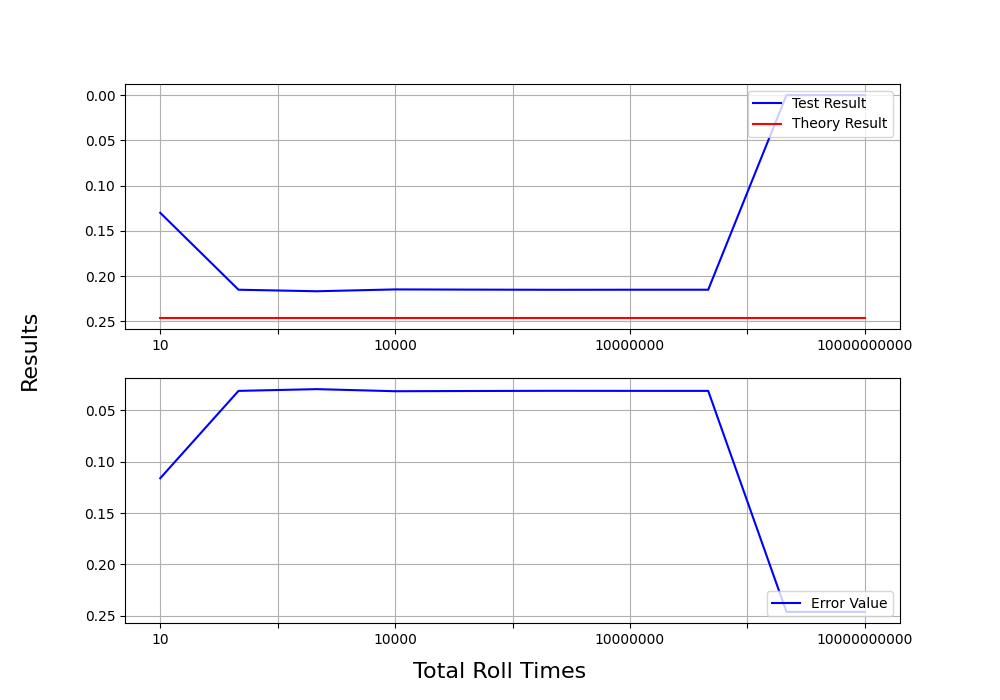
\includegraphics[height=6cm, keepaspectratio]{height1.png}
    \caption{回数-実験確率グラフ}
    \label{graph:height1}
\end{figure}
このグラフから見ると, 10万回以上の中で26%は条件で並んでいるということがわかる.
回数を増やしても, 実験値は理論値に近づくということが言える. 

\section{BINGOシムレーション}
このシムレイションは3っつの確率を求める.
\begin{enumerate}
    \item 最短回数(4回)で当たりとなる確率をシミュレーション
    \item 7回以内で当たる確率をシミュレーション
    \item 当たりとなる最も遅いゲーム回数とそのような状態の発生確率をシミュレーション
\end{enumerate}

\subsection{コードリスト}
このプログラムは6っつの関数がある. 全体的にはBINGOカードを生成し, BINGOをシムレイションを行い, 一回ゲーム何回にBINGOかをそれぞれの変数に入れる. これをN回で繰り返す. 

まずは [\textit{Code line 1-10}]~create\_bingo(int* bingo)関数ではBINGOの1次配列を生成し, 1から75までの値を持つ, [\textit{Code line 12-16}]~tester配列を生成する. tester配列は同じ値がBINGOカードに出ないように, 出た値を配列に1にする, まだ出ない値は0にする. それで[\textit{Code line 18-42}]~create\_numarray(int *bingo, int *test)関数は実際にBINGOカードを生成する関数である. コードリストは Listing\ref{createbingo}に掲載される.

\begin{lstlisting}[
    style=CStyle, 
    caption=$create\_bingo()$関数コードリスト,
    captionpos=t,
    label=createbingo]
    void create_bingo(int* bingo) {

        int y,x;
        int *test;

        test = (int*)malloc(sizeof(int)*75);
        tester(test);
        create_numarray(bingo, test);
        free(test);
    }

    void tester(int *test) {
        int y,x;
        for(y = 0; y < 75; y++){
                test[y] = 0;
    }

    void create_numarray(int *bingo, int* test) {
        int num, index;
        int x,y;
        int min, max;
        min = 1; max = 15;
        for (x = 0; x < N; x++){
        y = 0;
            while(1){
                index = rand()%(max-min+1) + min;
                num = index + 1;
                if(test[index] == 0){
                    bingo[y * N + x] = num;
                    test[index] = 1;
                    y++; 
                }
                if (y >= 5) {
                    max += 15;
                    min += 15;
                    break;
                }
            }
        }
        bingo[2*N+2] = 0;
    }    
}

\end{lstlisting}
\vspace{10pt}
そして, Listing\ref{playbingo}のなかで, [\textit{Code line 1-25}]~play(int *bingo, int* counter)関数では実際にゲームがシムレイションされる. まずは同じtest配列を生成し,while関数にはいり, ランダムな値を生成し, その値がtest配列に1ならば, もう一度値を生成する. BINGOカードにある当たった値を0にする. それで[\textit{Code line 27-60}]~check(int* bingo)関数でBINGOかどうか判定する. BINGOがあったら1を返すが当たらなかったら繰り返す. 

\begin{lstlisting}[
    style=CStyle, 
    caption=play()関数コードリスト,
    captionpos=t,
    label=playbingo]
    int play(int *bingo, int* counter){

        int i, number;
        int *test;
        test = (int*)malloc(sizeof(int)*75);
        tester(test);    
    
        while(1) {
            number = rand()%75 + 1;
            if(test[number] != 1){
                *counter += 1;
                test[number] = 1;
                for(i = 0; i < N*N; i++){
                    if(bingo[i] == number){
                        bingo[i] = 0;
                        
                    }
                }
                if(check(bingo) == 1) {
                    free(test);
                    return 1;
                }
            }else continue;
        }  
    }

    int check(int *bingo){
    int x, y;

    //horizontal
    for(y = 0; y < N; y++){
        if (bingo[y * N + 0] == bingo[y * N + 1] && 
            bingo[y * N + 1] == bingo[y * N + 2] &&
            bingo[y * N + 2] == bingo[y * N + 3] &&
            bingo[y * N + 3] == bingo[y * N + 4] &&
            bingo[y * N + 4] == bingo[y * N + 1] ) return 1;
    }

    //vertical
    for(x = 0; x < N; x++){
        if(bingo[x + N * 0] == bingo[x + N * 1] &&
           bingo[x + N * 1] == bingo[x + N * 2] &&
           bingo[x + N * 2] == bingo[x + N * 3] &&
           bingo[x + N * 3] == bingo[x + N * 4] &&
           bingo[x + N * 4] == bingo[x + N * 0]) return 1;
    }

    //diagonal left-right
    if (bingo[0] == bingo[6] &&
        bingo[6] == bingo[12] && 
        bingo[12] == bingo[18] && 
        bingo[18] == bingo[24]) return 1;

    //diagonal right-left
    if (bingo[4] == bingo[8] &&
        bingo[8] == bingo[12] && 
        bingo[12] == bingo[16] && 
        bingo[16] == bingo[20]) return 1;

}
\end{lstlisting}

\subsection{最短回数(4回)で当たりとなる確率}
サイトから引用し, 最短回数の理論値は0.0000032910である\cite{Bingo-確率}. グラフ\ref{graph:below4}は実験結果とリ論調の比べグラフである.

\begin{figure}[h]
    \centering 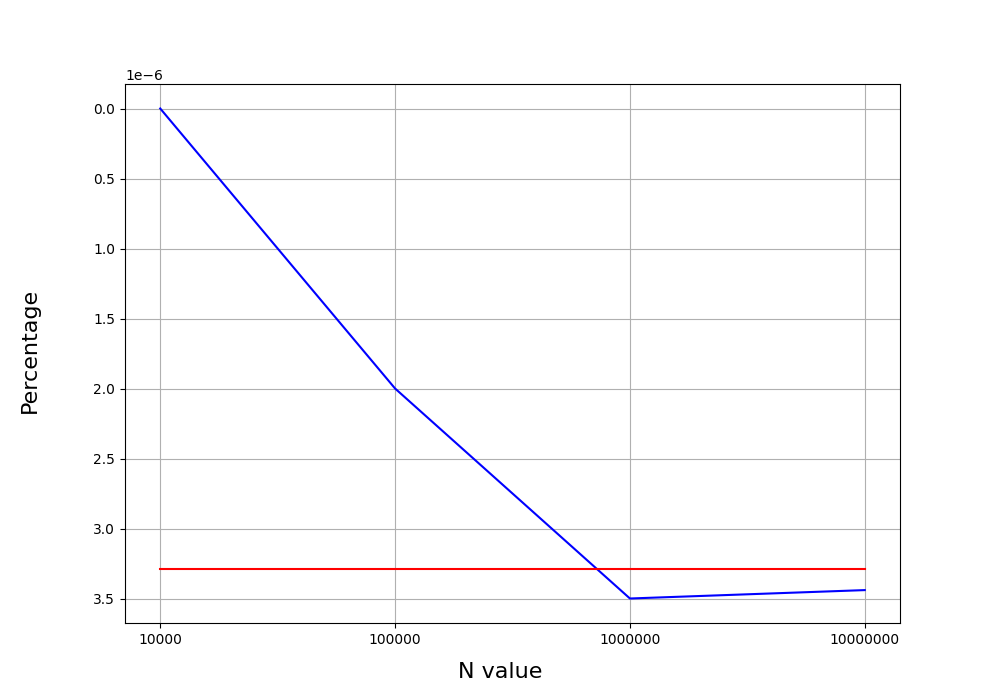
\includegraphics[height=6.5cm, keepaspectratio]{bingo4.png}
    \caption{回数-実験確率グラフ(最短回数)}
    \label{graph:below4}
\end{figure}

実験結果より, 100万回ゲームの中で34回起きる. つまり294117ゲームの中で少なくとも1回起きる. 

\subsection{7回以内で当たる確率}
サイトから引用し, 最短回数の理論値は0.0000727720である\cite{Bingo-確率}. グラフ\ref{graph:below7}は実験結果とリ論調の比べグラフである.

\begin{figure}[h]
    \centering 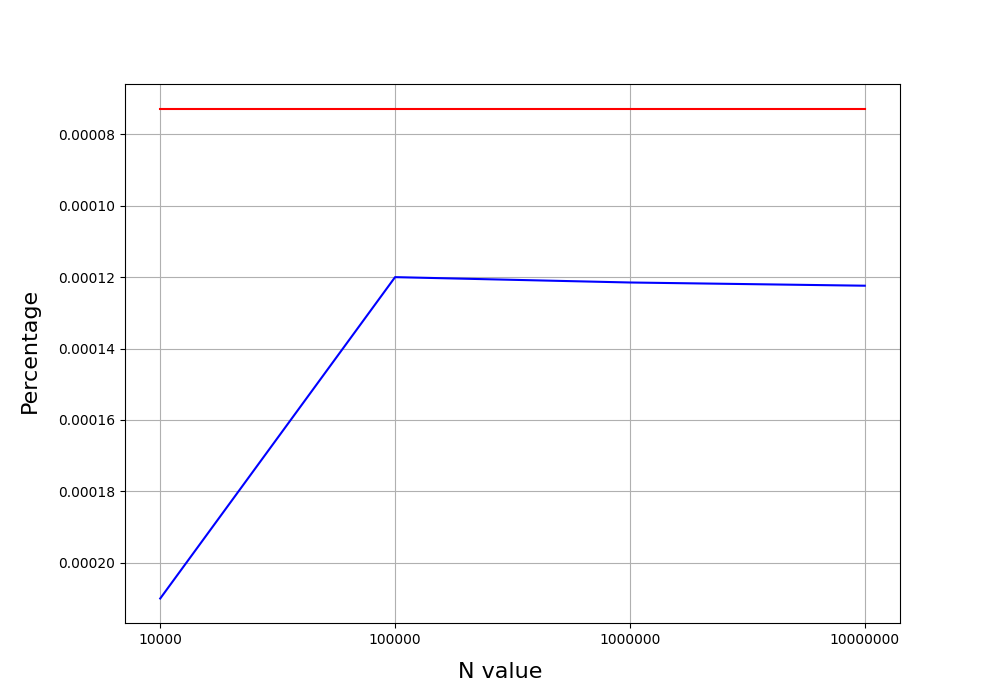
\includegraphics[height=6.5cm, 
keepaspectratio]{bingo7.png}
    \caption{回数-実験確率グラフ(7回)}
    \label{graph:below7}
\end{figure}

実験結果より, 100万回ゲームの中で1200回起きる. つまり8333ゲームの中で少なくとも1回起き
る. 

\subsection{る最も遅いゲーム回数で当たる確率}
サイトから引用し, 最短回数の理論値は0.0000013905である\cite{Bingo-確率}. グラフ\ref{graph:below71}は実験
結果とリ論調の比べグラフである.

\begin{figure}[h]
    \centering 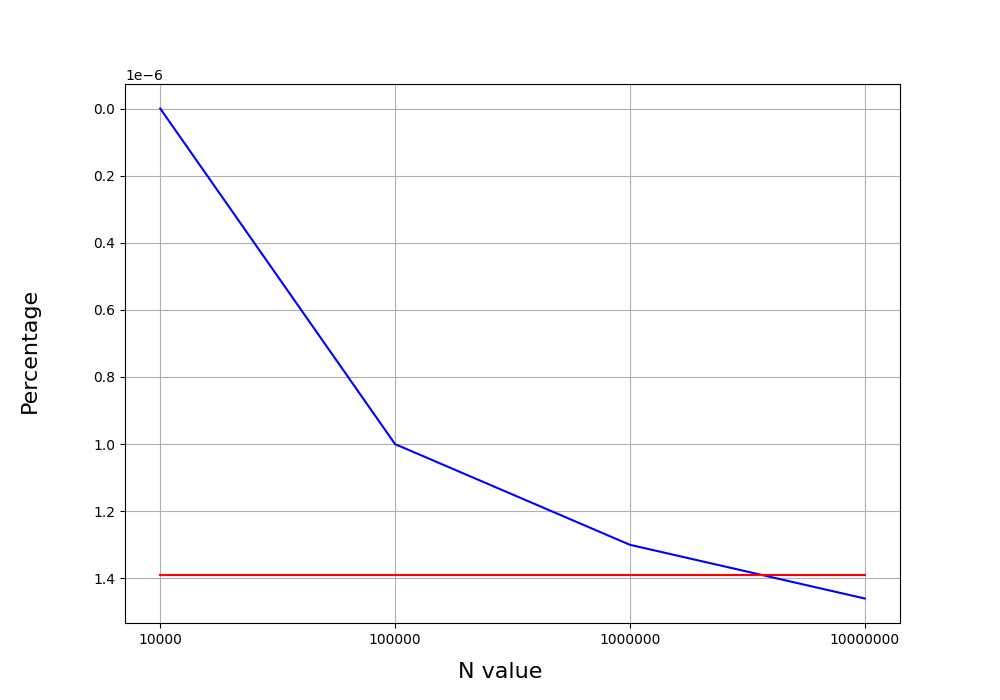
\includegraphics[height=6.5cm, 
keepaspectratio]{bingo71.png}
    \caption{回数-実験確率グラフ(7回)}
    \label{graph:below71}
\end{figure}

実験結果より, 100万回ゲームの中で13回起きる. つまり769230ゲームの中で少なくとも1回起き
る. 

\pagebreak
\section{感想}
今日の鎌田のプレゼンテーションは良かったと思います. プレゼンテーションの内容が理解できやすかった. 回数シムレイションはとても多く, ちゃんと理論値に近づくまたは精度が高いということを言えます. でも, スライドの背景のせいか, 内容は少し見づらくなりました. スライドの画像も少し大きくすれば良かった. 

\begin{thebibliography}{99}
\bibitem{Bingo-確率}
Bingo Probabilities — Part One \url{https://wizardofodds.com/games/bingo/probabilities/1/}
\end{thebibliography} 

\end{document}

